\documentclass[a4paper]{article}
\usepackage[utf8]{inputenc}

\newcommand{\newpar}{\vspace{.3cm}\noindent}

\title{\vspace{5cm} \Huge Linkages}
\author{Karel Smets, Mathias Schietecat}
\date{April 2021}

\usepackage[dutch,english]{babel}
\usepackage{natbib}
\usepackage{graphicx}
\usepackage{wrapfig} 
\usepackage{amsmath}
\usepackage{amssymb}
\usepackage{caption}
\usepackage{subcaption}
\usepackage{lscape}
\usepackage{multicol}
\usepackage{hyperref}
\usepackage{anyfontsize}
\usepackage{changepage}
\usepackage{textcomp}
\usepackage{float}


\def\mydate{December 2021}

% Paginamarges
\usepackage{geometry}
\geometry{a4paper,
total={170mm,257mm},
left = 30mm,
top= 30mm,
right=30mm,
bottom=30mm
}

\begin{document}

\begin{titlepage}
\date{April 2021}
    \begin{center}
        \vspace*{1cm}
        
        \Huge
        Control Theory 
        
        \vspace{0.5cm}
        \Huge
        Mecotron Assignment: Swivel
        
        \vspace{1.5cm}
        \large
        Team 6:\\
        Mathias Schietecat\\
        Karel Smets\\
        \vspace{1cm}
        \mydate 
        
        \vfill
        
        \begin{figure}[h]
        \centering
        \includegraphics[scale=1]{Illustrations/KULEUVEN_CMYK_LOGO.jpg}
        \end{figure}
        
        \vspace{1cm}
        \large
        Departement Werktuigkunde\\
        Professor J. Swevers\\
        Professor G. Pipeleers\\
    \end{center}
\end{titlepage}

\newpage

\setcounter{page}{2}
\tableofcontents

\newpage

\section{Assignment 1: motor identification}

\subsection{Model structure}
\subsubsection{Discrete model structure}
% state first discrete tf representation
% elaborate on how it comes to be
% = state physical laws and discuss

A third order model (denominator order three) with a second order numerator is used to represent the behaviour of the DC motor. The general format of this model is shown below:
\begin{equation}
    G(z)=\frac{b_{0} z+b_{1}}{a_0 z^{3}+a_{1} z^{2}+a_{2} z}
    \label{eq:model}
\end{equation}
This representation is based upon a combined mechanical and electrical representation of the  of the motor. The electrical behaviour is moddeled as follows:

\begin{equation}
    V(s)-R_{a} I(s)-L s I(s)=K_{e} \phi \omega(s)
    \label{eq:electrical}
\end{equation}

\newpar
The mechanical part also contains the wheel (inertia). This is given by:

\begin{equation}
    J s \omega(s)=T(s)-T_{L}(s)-C \omega(s)
    \label{eq:mech}
\end{equation}

\newpar
The electrical and mechanical representations are coupled through the torque-current relation \autoref{eq:torquecurrent} and the back emf \autoref{eq:backemf}.
\begin{center}
    \begin{tabular}{p{5cm}p{5cm}}
        \begin{equation}
            T(s)=K_{t} \phi I(s)
            \label{eq:torquecurrent}
        \end{equation}
        &  
        \begin{equation}
            V_{EMF}(s)=K_{e} \phi \omega(s)
            \label{eq:backemf}
        \end{equation}
        
    \end{tabular}
\end{center}

\newpar
The result is a second order continuous time transfer function which relates the rotor speed to the terminal voltage. The denominator has to real poles, caused by the inertial time constant and the one caused by the rotor coil inductance. The electrical delay is smaller than the mechanical one and can be omitted. Though, this is not done because leaving it in gives an noticeable improvement in the model behaviour as will be seen later.

\newpar
The discretization of this transfer function is done using the ZOH-method. Due to cancellations in the numerator and denominator upon multiplication of the ZOH factor \((1-z^{-1})\) with the discrete representation, the discrete motor model is of order two with two zeros. During the identification proces, the second zero turned out to be always negligible. Therefor the number of zeros in the model was reduced to one. 

\newpar
The discrete motor model differs from the system as seen by the controller due to the output delay caused by MicroOS. This is accounted for by introducing a factor \(z^{-1}\) in the transfer function, making it of the form represented in \autoref{eq:model}.
% the above paragraph to much of an explenation?

\newpar
The above procedure is graphically represented in \autoref{fig:modelphysics}

% include torque disturbance model?? --> part of ARX no?

\subsubsection{Inputs, outputs, and their units}
The input of the model is the motor terminal voltage \(V(s)\) expressed in \([V]\) (volt). The output is the angular velocity of the rotor \(\omega(s)\) in \([rad/s^2]\).

\subsection{Identification of motor-wheel system} \label{motor-wheel}
\subsubsection{Excitation signal}

While identifying the system, it is important to make sure the excitation signal is sufficiently rich. This condition is called the \emph{persistency of excitation}. Meeting it insures that all the the modes of the DC motor are excited and thus observable in the output. For this reason, we choose to excite the system with a block-pulse of constant voltage as shown in \autoref{fig:excitationSignal6V}. This signal contains a broad enough frequency range.

  \begin{figure}[H]
      \makebox[\textwidth][c]{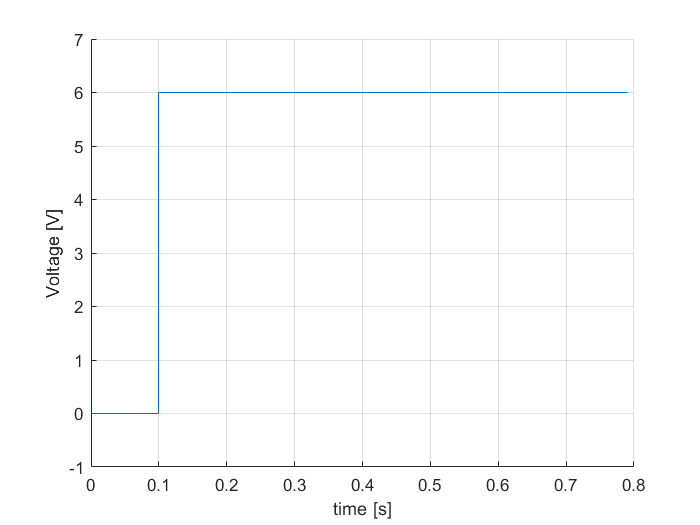
\includegraphics[width=0.5\textwidth]
      {figs/assign1/Q2/excitationSignal6V.png}}
      \caption{Excitation signal step input of 6V}
      \label{fig:excitationSignal6V}
  \end{figure}

\newpar
The block-pulse as input is repeated 5 times in time. This allows us to to average out the response of the system, in order to minimize the influence of noise and other disturbances. On top of that, different voltages are fed into the system. We chose for 3V, 6V, 9V and 12V to have a broad coverage of the voltage range. This will allow us later on to check the linearity of our system. 

\subsubsection{Obtaining system parameters}
To obtain the system parameters, we first have a look at difference equation following from the proposed model (\autoref{eq:model}) in \autoref{eq:difference equation}. Note that the internal delay in MicroOS is also visible here, because \(\omega[k]\) is independent of \(u[k]\). Its dependency starts at \(u[k-1]\).

\begin{equation}
    \omega[k] + a_2 \omega[k-1] + a_1 \omega[k-2] = b_2 u[k-1] + b_1 u[k-2] + b_0 u[k-3]
    \label{eq:difference equation}
\end{equation}

\newpar
Error criterion that this expression minimizes??

\newpar
In \autoref{tab:location_Sys_31z} the location and accompanying frequency of the different poles and zeros are displayed.

\begin{center}
    \begin{tabular}{ |c|c|c|c|c|}
    \hline
    Zero/Pole & Location & \omega_n{[}rad/s{]} & \omega_n{[}Hz{]} & \zeta  \\
    \hline
    z1        & -0.816    & 315      &  50.13   & 0.0647           \\
    \hline
    p1        & 0         & /        & /        & /               \\
    \hline
    p2        & -0.243    & 344      & 54.75    & 0.41             \\
    \hline
    p3        & 0.514     & 66.6     & 10.60    & 1       \\ 
    \hline
    \end{tabular}  
    \captionof{table}{location and frequency of poles and zeros in the fitted system}
    \label{tab:location_Sys_31z}
\end{center}

\subsubsection{Filtering}
While measuring the response of the system to the excitation signal, we should keep in mind that the measurements are not perfect. Noise will be included into these measurements. Typically this noise will be in the high frequency range of the output signal. This noise is unwanted and we should try to remove it. 

\newpar
Another reason to filter the measured date, is due to the fact that the least-squares estimate method has an intrinsic high-pass character. This means that the identification method gives more 'weight' to the high frequency errors than the errors at lower frequency. However, most of the noise is situated at high frequencies. For this reason, it is advisable to filter the data with a low-pass filter to compensate this high-pass characteristic of the estimation method. It is important that both the output and input data are sent through the same filter, to make sure that the relation between the filtered signals does not change. 

\newpar
As mentioned before, we want to suppress the high pass character of the estimation method. This means that the filter should have at least the same order as the model being proposed during estimation. If it is desired to further suppress the high frequency measurement noise, the order of the filters should be higher than the order of the model. We chose to use a butterworth filter of order 4 and cutoff frequency of $70\pi rad/s$ as these gave the best results, minimizing the errors of the model compared to the measurements. 

\newpar
The result of the model estimation after filtering using the same amount of poles and zero's is displayed in \autoref{tab:location_Sys_31z_f}. It is clear that the location of the poles and zeros have shifted a bit. This is also visualised in the pole-zero maps of the identified model with and  without filter in \autoref{fig:pzmap}.

\begin{center}
    \begin{tabular}{ |c|c|c|c|c|}
    \hline
    Zero/Pole & Location & \omega_n{[}rad/s{]} & \omega_n{[}Hz{]} & \zeta  \\
    \hline
    z1        & -0.632    & 317                 &  50.45    & 0.145         \\
    \hline
    p1        & 0         & /                   & /         & /          \\
    \hline
    p2        & -0.0375   & 454                 & 72,26     & 0.723         \\
    \hline
    p3        & 0.482     & 73                  & 11,62     & 0.482        \\ 
    \hline
    \end{tabular}  
    \captionof{table}{location and frequency of poles and zeros in the fitted system after filtering}
    \label{tab:location_Sys_31z_f}
\end{center}

\begin{figure}[H]
    \makebox[\textwidth][c]{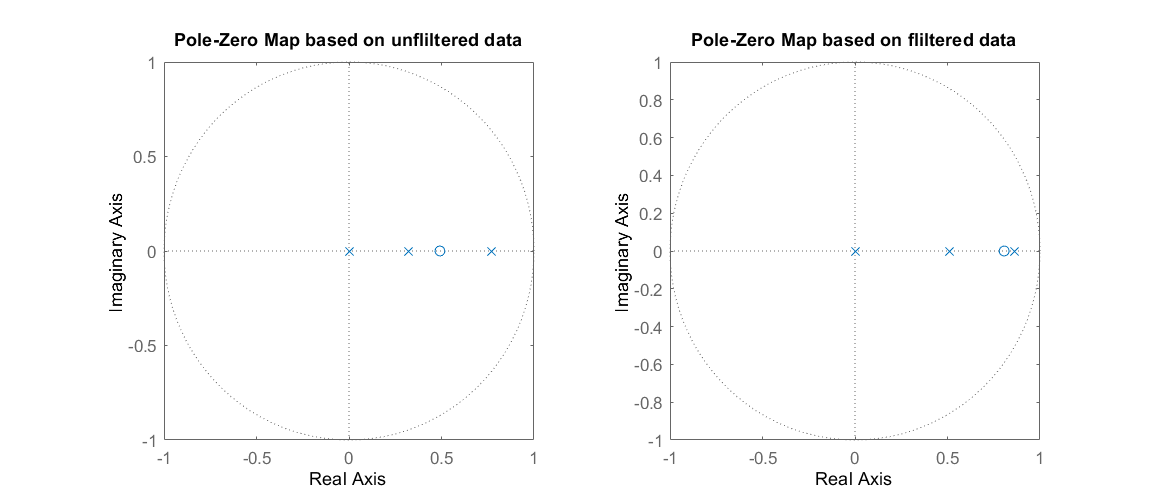
\includegraphics[width=1.2\textwidth]
    {figs/assign1/Q2/motor/pzmap}}
    \caption{Pole-zero map of identified model with(right) and without(left) filtering}
    \label{fig:pzmap}
\end{figure}

\subsubsection{Model validation}
After estimating a model, we can compare the identified model with the measured data. Both the measured and simulated outputs for a step input of 6V are displayed in \autoref{fig:StepResponse}. Also the errors between the simulated responses and the measured one is calculated and displayed in \autoref{fig:StepResponseError}

\newpar
As you can see, the difference between the filtered model and unfiltered is rather small. However, later on we will see that the model using filters performs slightly better when we calculate the model for the complete cart instead of the motors without load. Therefor we would select the model with that uses the filtered data.

\begin{figure}[H]
    \makebox[\textwidth][c]{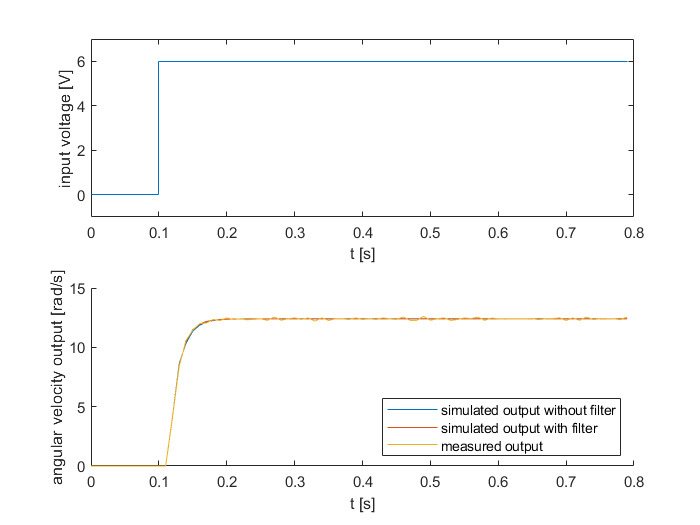
\includegraphics[width=1.0\textwidth]
    {figs/assign1/Q2/motor/StepResponse}}
    \caption{measured and simulated responses}
    \label{fig:StepResponse}
\end{figure}

\begin{figure}[H]
    \makebox[\textwidth][c]{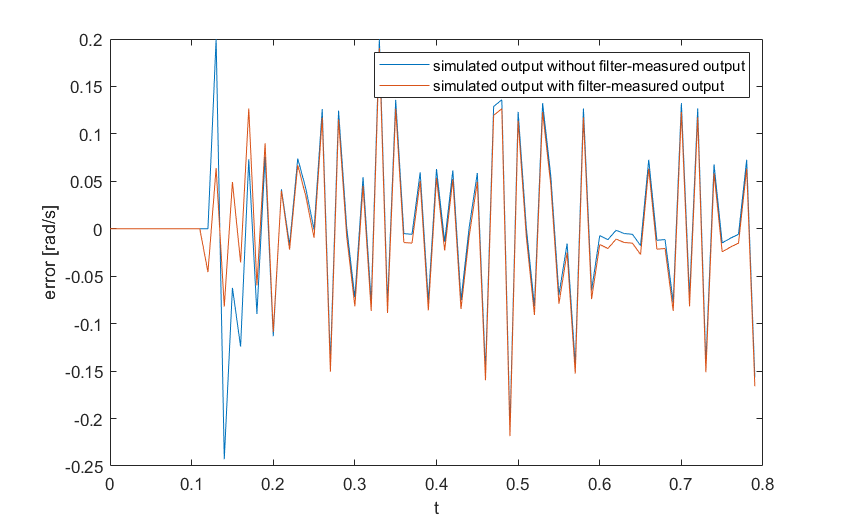
\includegraphics[width=1.0\textwidth]
    {figs/assign1/Q2/motor/error}}
    \caption{error between measured and simulated responses}
    \label{fig:StepResponseError}
\end{figure}

\newpar
The superposition principle:
Assume two arbitrary inputs $x_1(t)$ and $x_2(t)$ and working with a system H(s), the following is valid:

\begin{equation}
    y_1(t) = H\{x_1(t)\}
\end{equation}
\begin{equation}
    y_2(t) = H\{x_2(t)\}
\end{equation}

\newpar
If H(s) is a linear system, it must satisfy:
\begin{equation}
    \alpha y_1(t) + \beta y_2(t) = H\{\alpha x_1(t)+\beta x_2(t)\}
\end{equation}

\newpar
We can use the equation above to check if the cart is indeed linear, as assumed by approximating it by a linear model. As the conditions says, the sum of the responses should be the same as the response to the sum of the inputs.  This is visualised in \autoref{fig:linearityCheck}. For example: we can compare the response of a 12V input with twice the response of a 6V input, or 4 times the response of a 3V input. As you can see, the responses don't coincide as it should be the case in a perfectly linear system. These nonlinearities in our system are a result of a couple aspects, e.g. eddy currents, hysteresis losses, frictional aspects and cogging torque. (cogging torque in a permanent magnet motor is due to the interaction between permanent magnets in the stator and the slot in the rotor)

\begin{figure}[H]
    \makebox[\textwidth][c]{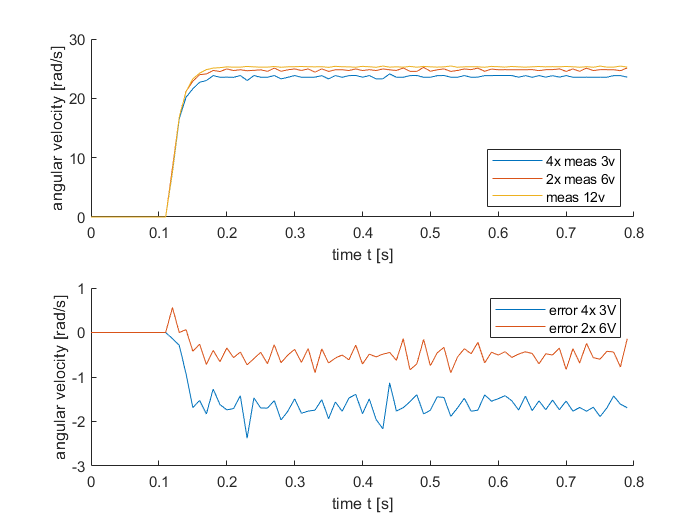
\includegraphics[width=0.8\textwidth]
    {figs/assign1/Q2/motor/linearityCheck.png}}
    \caption{Checking the superposition principle}
    \label{fig:linearityCheck}
\end{figure}

\newpar
However, the violations on the linearity principle are rather small. Approximating the system by a linear estimation is still a valid, and will give us sufficiently good results. 

\subsection{Identification of cart}
\subsubsection{Comparing to motor-wheel model}
The cart is placed onto the ground and step responses are measured an in section \ref{motor-wheel}. Steps of three, six, nine and twelve volts are administered to the motor. Below, in \autoref{fig:loadunloadcompA}, the measured response is compared to the simulated one based on the six volt step data of motor A. \autoref{fig:loadunloadcompA} shows the same for motor B.

\begin{figure}[H]
    \makebox[\textwidth][c]{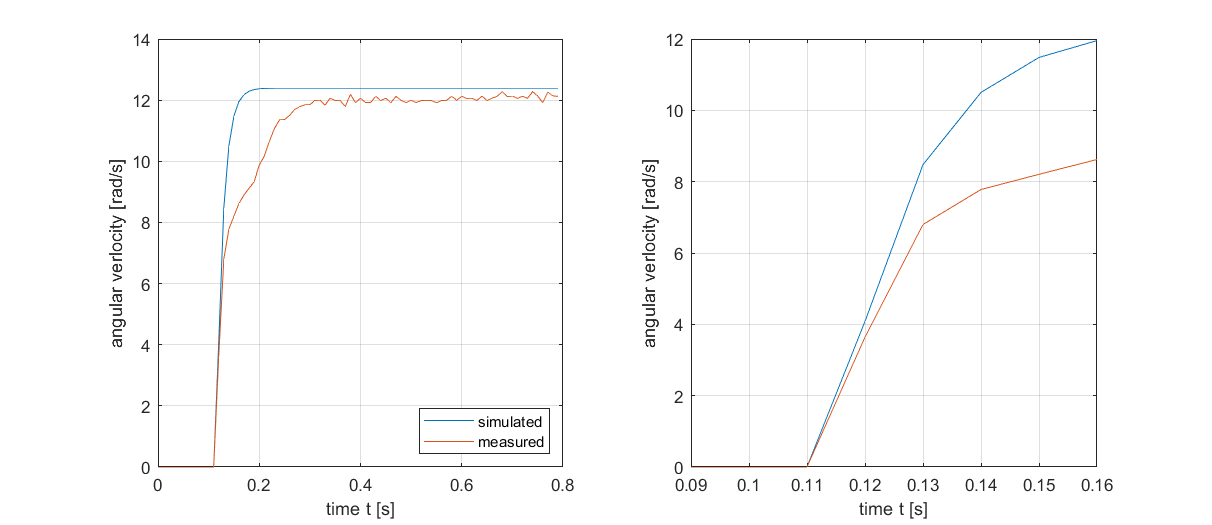
\includegraphics[width=1.0\textwidth]
    {figs/assign1/Q3/3a_motor_A.png}}
    \caption{left: Comparison of motor A response when on ground to the simulated response using the model motor-wheel system. right: enlargement of first part of transient.}
    \label{fig:loadunloadcompA}
\end{figure}

\begin{figure}[H]
    \makebox[\textwidth][c]{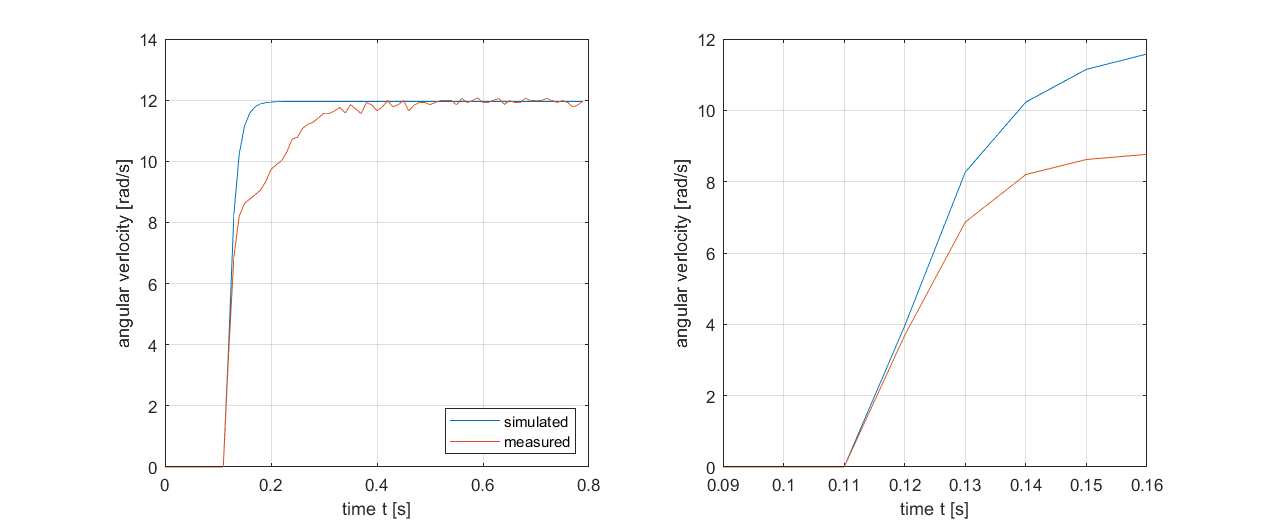
\includegraphics[width=1.0\textwidth]
    {figs/assign1/Q3/3a_motor_B.png}}
    \caption{left: Comparison of motor B response when on ground to the simulated response using the model motor-wheel system. right: enlargement of first part of transient.}
    \label{fig:loadunloadcompB}
\end{figure}

\newpar
The plots on the right show that the angular velocity is rising slower. This is to be expected because the inertia of the system has increased now that the cart itself is also moving. The impact on the steady state is negligible, because at constant speed the system inertia does not matter anymore (zero acceleration). In the measurement there is clearly a dip at the top of the rising edge. This dip is always present, becomes more extended in time for larger input step voltages and starts at approximately at the same time after the motor voltage is applied. This is shown in \autoref{fig:_mean_v}. Because the duration of the dip depends on the input voltage, it is non linear in nature an can not be incorporated in the linear model.

\newpar
The origin of these dips is probably slip. The larger the applied step, the higher the acceleration, causing the slip to continue longer. During slip the motor is loaded more due to the frictional force between the tire and ground. This explains the velocity increase when the slipping stops.

% te lange text, nuance meer verleggen naar dat de dip slecht word gevolgd door het motor-wiel model mits die er eerst niet was en het dus beter kan.

\begin{figure}[H]
    \makebox[\textwidth][c]{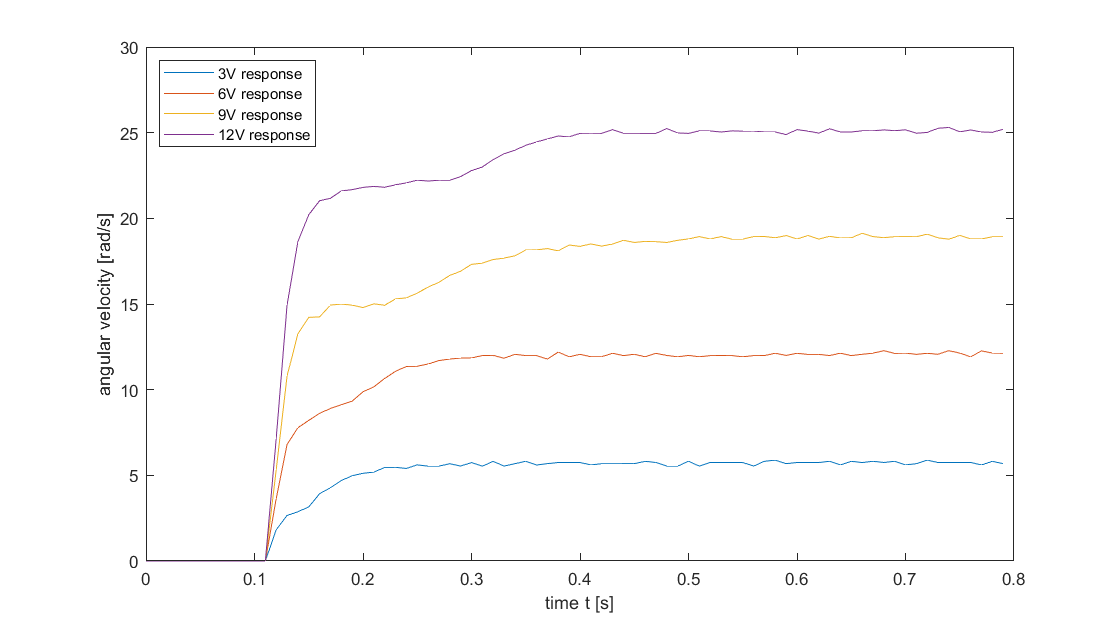
\includegraphics[width=1.0\textwidth]
    {figs/assign1/Q3/dips.png}}
    \caption{Motor angular speed caused by 3,6,9 and 12V step input (averaged over 5 measurements). The almoast linear increase in duration with the voltage is clearly visable.}
    \label{fig:_mean_v}
\end{figure}

\subsubsection{Re-identification}
The reidentified model parametres are:

\begin{center}
    \begin{tabular}{ |c|c|c|c|c|}
    \hline
    \multicolumn{5}{|c|}{motor A} \\
    \hline
     $a_0$ & $a_$ & $a_2$ & $b_0$ & $b_1$ \\
    \hline
    1 & -1.375 & 0.4417 & 0.6903 & -0.5566 \\
    \hline
    \multicolumn{5}{|c|}{motor B} \\
    \hline
     $a_0$ & $a_$ & $a_2$ & $b_0$ & $b_1$  \\
    \hline
    1 & -1.383 & 0.4548 & 0.6819 & -0.5404 \\
    \hline
    \end{tabular}  
    \captionof{table}{Estimated parameters for motor-wheel-cart model, based upon 6V step response measurements.}
    \label{tab:location_Sys_31z_f}
\end{center}

\begin{center}
    \begin{tabular}{ |c|c|c|c|c|}
    \hline
    \multicolumn{5}{|c|}{motor A} \\
    \hline
     $a_0$ & $a_$ & $a_2$ & $b_0$ & $b_1$ \\
    \hline
    1 & -0.444 & -0.01805 & 0.6804 & 0.43 \\
    \hline
    \multicolumn{5}{|c|}{motor B} \\
    \hline
     $a_0$ & $a_$ & $a_2$ & $b_0$ & $b_1$  \\
    \hline
    1 & -0.4466 & 0.009759 & 0.6595 & 0.4238 \\
    \hline
    \end{tabular}  
    \captionof{table}{Estimated parameters for motor-wheel model, based upon 6V step response measurements.}
    \label{tab:location_Sys_31z_f}
\end{center}

\newpar
The corresponding locations of the discrete poles and zeros are:

\begin{center}
    \begin{tabular}{ |c|c|c|c|}
    \hline
    \multicolumn{4}{|c|}{motor A} \\
    \hline
    Zero/Pole & Location & Frequency{[}rad/s{]} & Frequency{[}Hz{]}  \\
    \hline
    z1        & 0.806    & 21.5                &  3.42           \\
    \hline
    p1        & 0         & /                   & /                 \\
    \hline
    p2        & 0.511   & 67.1                 & 10.68            \\
    \hline
    p3        & 0.864     & 14.7                  & 2.34 \\ 
    \hline
    \hline
    \multicolumn{4}{|c|}{motor B} \\
    \hline
    Zero/Pole & Location & Frequency{[}rad/s{]} & Frequency{[}Hz{]}  \\
    \hline
    z1        & 0.792    & 23.3                &    3.71         \\
    \hline
    p1        & 0         & /                   & /                 \\
    \hline
    p2        & 0.539   & 61.7                 &   9.82          \\
    \hline
    p3        & 0.843     & 17.1                  & 2.72           \\ 
    \hline
    \end{tabular}  
    \captionof{table}{Location and frequency of poles and zeros of the identified motor wheel-cart system.}
    \label{tab:location_Sys_31z_f}
\end{center}

\newpar 
The poles have become slower compared to those of the motor-wheel model. The system dynamics have thus become slower. This is in line with the expectations. As said before, the inertia of the system has increased due to the mass of the cart that now has to be moved to. The larger inertia makes the system respond slower.

\newpar
For completeness, the simulated step response using the new models is compared to the measurements in \autoref{fig:cartmodelvalidation}. Comparing this to the results for motor A and B in \autoref{fig:loadunloadcompA} and \autoref{fig:loadunloadcompB}, the new model is now much better following the transient.

\begin{figure}[H]
    \makebox[\textwidth][c]{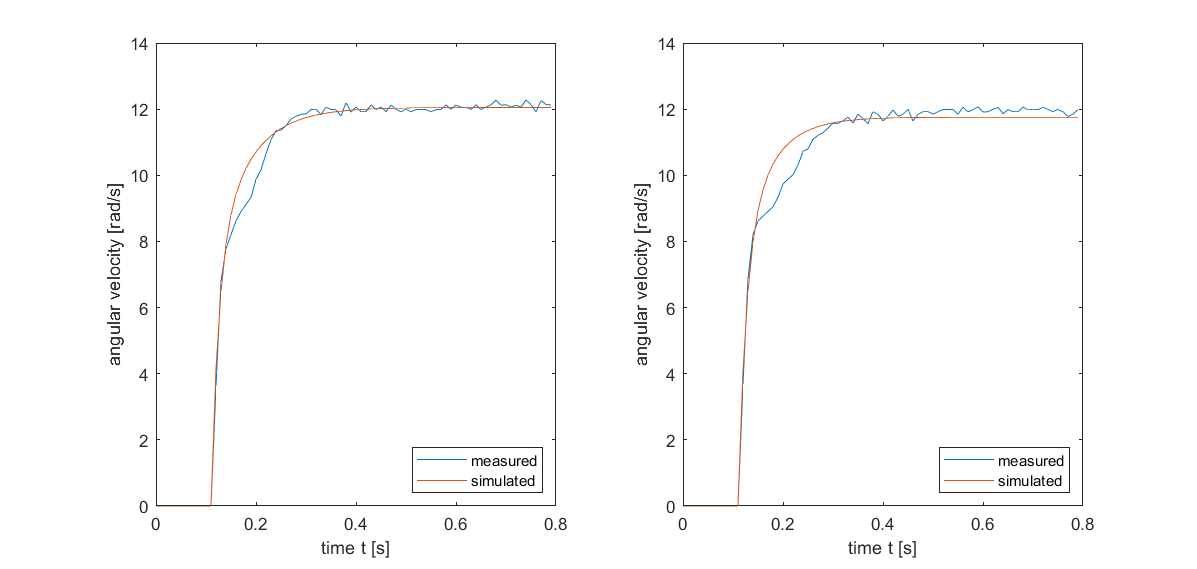
\includegraphics[width=1.0\textwidth]
    {figs/assign1/Q3/cart_identification_validation.png}}
    \caption{Motor A and B angular speed step response (6V step) next to simulated responses.}
    \label{fig:cartmodelvalidation}
\end{figure}

% ------------------------------------------------------------------
% -- assignment 2 --
% ------------------------------------------------------------------

\section{Assignment 2: velocity control of the cart}

\subsection{Design of velocity controllers for motor A and B}

\subsubsection{Controller type and requirements}

The initial requirements are:

\begin{itemize}
  \item Open loop system type 1 (at least) to get \(e_{ss} = 0\).
  \item Phase margin of 50° or higher to reduce the overshoot sufficiently
  \item Maximum bandwidth achievable given the above requirements to obtain fast responding system.
\end{itemize}

\newpar
The controller will be at least a PI controller. The I part is needed to get an type 1 open loop system. The P part is needed to achieve a large bandwidth. This PI controller can be placed in series with a Lead compensator to achieve an ever higher bandwidth for the same phase margin.

\subsubsection{Design process and parameters}

The PI controller (using Tustin discretization) is represented as:

\begin{equation}
    C(z) = Ki \left( 1 + \frac{Ts}{2Ti}\frac{z+1}{z-1}\right)
\end{equation}

\newpar
Using a phase margin of 80° and a safety margin of 15° (to anticipate the phase lag introduced by the PI controller), the frequency is sought at which the phase of the identified system becomes:

\begin{equation}
    \phi = -180° + 80° + 15°
\end{equation}

\newpar
The corresponding frequency \(\omega_{c}\) is used to:

\begin{itemize}
    \item determine Ti as 
        \begin{equation}
            Ti = \frac{\tan \left( \frac{pi}{2} - \frac{15° pi}{180} \right)}{\omega_{c}}
        \end{equation}
    \item determine the physical system magnitude \( |G(\omega_{c})| \), with \(G(z)\) the discrete motor-wheel-cart system.
    \item determine the magnitude of the PI controller \( |C(\omega_{c})| \), with \(Kp = 1\) and \(Ti\) as calculated above.
\end{itemize}

\newpar
\(Kp\) is then calculated as \(Kp = \frac{1}{|G(\omega_{c})||C(\omega_{c})|} \), to get gain crossover at \(\omega_{c} \) in the loop gain. For completeness \(Ki\) is defined as \(Ki = \frac{Kp}{Ti} \).

\newpar
The trade-offs involving the design parametres are the following:

\begin{itemize}
    \item Kp: Enlarging the value of will shift the gain cross-over frequency wc of the open loop system to higher frequencies. This increases the bandwith of the system, making the system respond faster. At the same time the phase margin decreases because of the increasing phase lag of the open loop system at higher frequency, thus increasing the overshoot.
    \item Ti: The integration time Ti determines the location of the break frequency of the PI controller and thus the location of the phase transition. To keep the phase margin at gain crossover as large as possible, Ti should be made large to shift the phase lag of the PI controller to lower frequencies. The downside of doing this, is that the low frequency gain gets reduced, reducing the integration action, making the closed loop system slower.
\end{itemize}

\newpar
The open loop bode plot is displayed in \autoref{fig:2_openloopbode}.

\begin{figure}[H]
    \makebox[\textwidth][c]{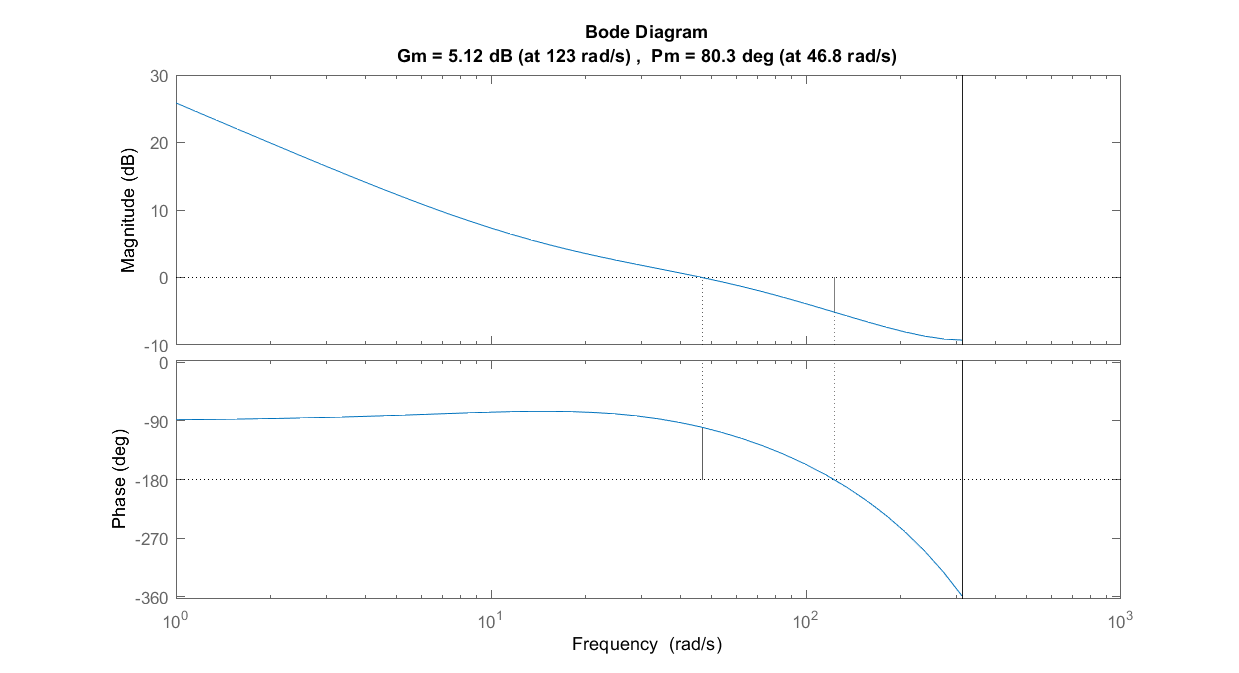
\includegraphics[width=1.0\textwidth]
    {figs/Q2_1/openloopbode.png}}
    \caption{Bode diagram of open loop system, designed phase margin and gain crossover indicated.}
    \label{fig:2_openloopbode}
\end{figure}

\newpar
The closed loop bode plot is displayed in \autoref{fig:2_closedloopbode}

\begin{figure}[H]
    \makebox[\textwidth][c]{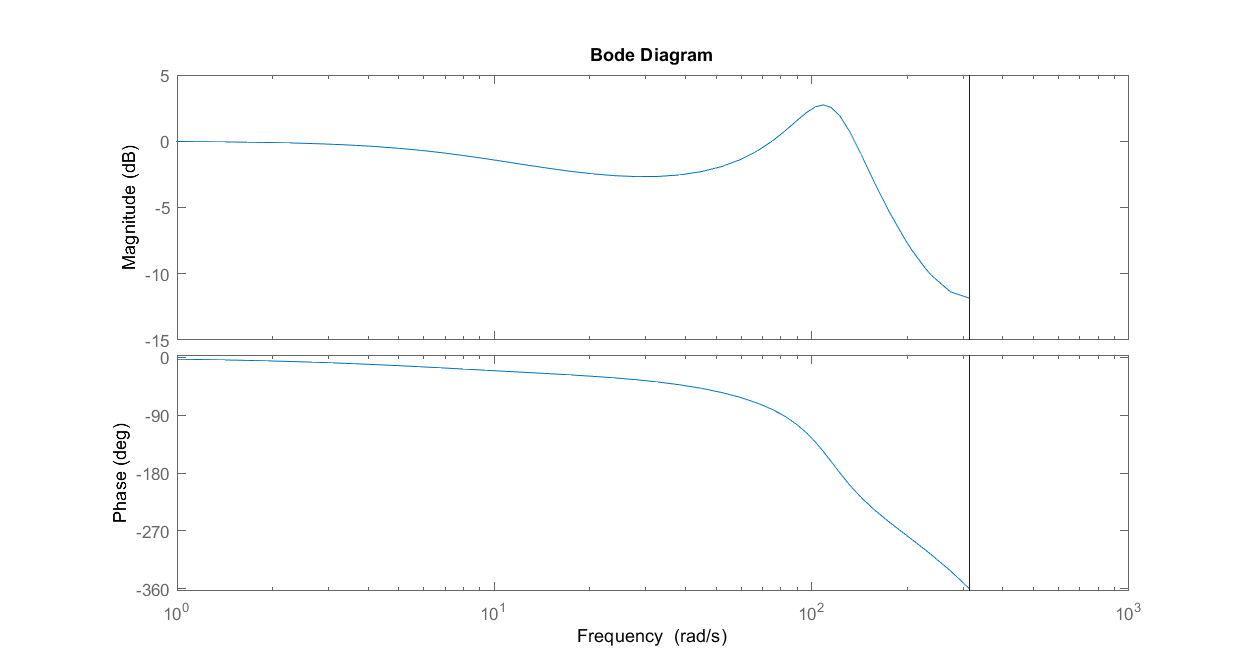
\includegraphics[width=1.0\textwidth]
    {figs/Q2_1/closedloopbode.png}}
    \caption{Bode diagram of closed loop system.}
    \label{fig:2_closedloopbode}
\end{figure}

\subsubsection{Bandwidth limitations}
Max theorethical bandwith is niquist freq = freq of fastest alternating digital !! output signal 


\subsection{Experimental validation of the controller}
\subsubsection{Controller performance}

\begin{figure}[H]
    \makebox[\textwidth][c]{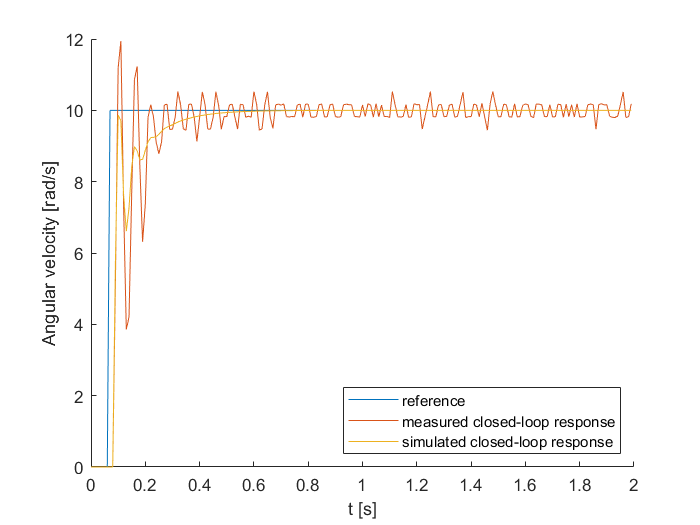
\includegraphics[width=0.8\textwidth]
    {figs/Q2_1/closed_loop_response.png}}
    \caption{The measured and simulated response of the closed-loop system}.
    \label{fig:closed_loop_response}
\end{figure}

\begin{figure}[H]
    \makebox[\textwidth][c]{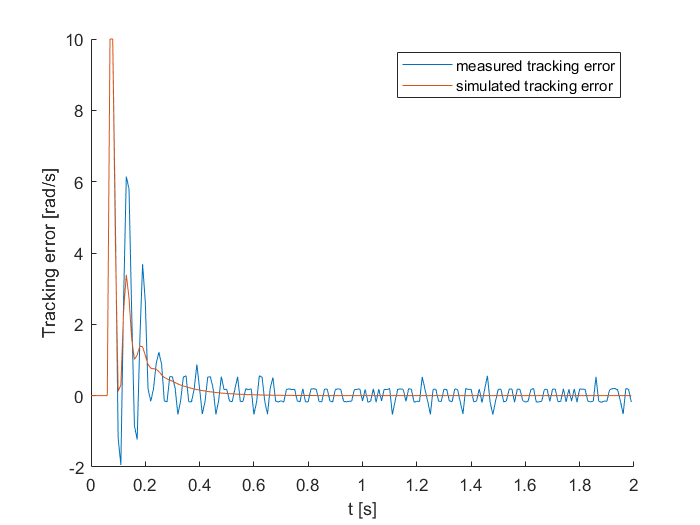
\includegraphics[width=0.8\textwidth]
    {figs/Q2_1/tracking_error.png}}
    \caption{The measured and simulated tracking error of the closed-loop system.}
    \label{fig:tracking_error}
\end{figure}

\begin{figure}[H]
    \makebox[\textwidth][c]{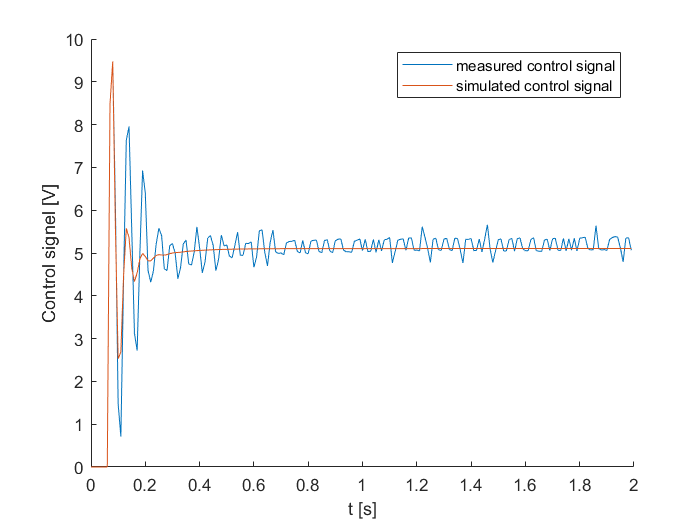
\includegraphics[width=0.8\textwidth]
    {figs/Q2_1/control_signal.png}}
    \caption{The measured and simulated control signal of the closed-loop system.}
    \label{fig:control_signal}
\end{figure}

\subsubsection{Constant force disturbance}
We can a apply a constant force disturbance by letting the cart drive up or downhill from a slope. This way, gravitational force will supply a constant force pulling the cart down. This disturbance $d(t)$ enters the system behind the plant, our cart as illustrated in \autoref{fig:disturbance_BlockDiagram}. $D(t)$ first passes throught the system $G_d(s)$ to convert this constant force into an influence on the velocitiy of the cart. 

\begin{figure}[H]
    \makebox[\textwidth][c]{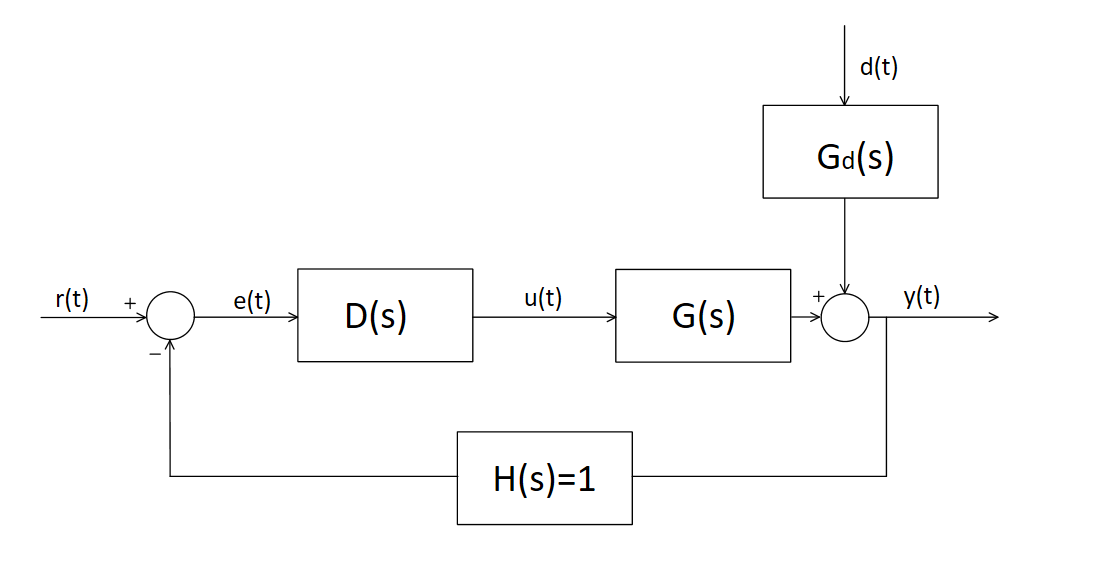
\includegraphics[width=0.8\textwidth]
    {figs/Q2_1/disturbance_block_diagram.png}}
    \caption{Block diagram of the complete system, including the constant force disturbance.}
    \label{fig:disturbance_BlockDiagram}
\end{figure}



\newpar
As is made visible in the figs.... the implemented controller is still able to track the reference despite the disturbance. This essentially is the goal of a good controller. The steady state error $e_{ss}$ eventually becomes zero, as was one of the requirements of our controller.


\section{Assignment 3: state feedback and state estimate}
\subsection{State feedback controller design}
\subsubsection{state equation}

The general continuous-time state equation is shown in \autoref{eq:general state space}, with $x$ the states of the system, and $u$ the inputs.
    \begin{equation}
        \dot{x} = Ax + Bu
        \label{eq:general state space}
    \end{equation}

\newar 
In our case of the cart, this converts itself into \autoref{eq:CT state space}, where $u$ is now substituted by velocity $v$ of the cart.
    \begin{equation}
        \dot{x} =  v
        \label{eq:CT state space}
    \end{equation}
\newar 
So $A=0$ and $B=1$ . However, to make the system implementable, we convert the velocity $v$ into the product of $R\omega$, with R the radius of the wheels and $\omega$ the rotational speed of the wheels. The result is then \autoref{eq:CT R state space}.
     \begin{equation}
        \dot{x} =  R\omega
        \label{eq:CT R state space}
    \end{equation}
\newar
So $A=0$ and $B=R\omega$
    
\newpar 
This state equation can then be discretized using a forward Euler scheme shown in \autoref{eq:forwardEuler}
    \begin{equation}
        \dot{x} = \frac{x[k+1] - x[k]}{T_s}
        \label{eq:forwardEuler}
    \end{equation}

\newar
Filling in the forward Euler scheme results in \autoref{eq:DT state equation}, our final discrete state equation.
    \begin{equation}
        x[k+1] = x[k] + RT_s\omega[k]
        \label{eq:DT state equation}
    \end{equation}

\newar
So $A=1$ and $B=RT_s$. 

\subsubsection{State feedback gain K} \label{subsec:gain K}
The pole of the discretized closed-loop system, shown in \autoref{} can be expressed by \autoref{eq:DT closed loop pole} and \ref{eq:CT closed loop pole}, both in discrete and continuous time. 

    \begin{align}
        \label{eq:DT closed loop pole}
        & p_d = 1-RT_sK \\
        \label{eq:CT closed loop pole}
        & p_c = \frac{ln(1-RT_sK)}{T_s}
    \end{align}

\begin{figure}[H]
    \makebox[\textwidth][c]{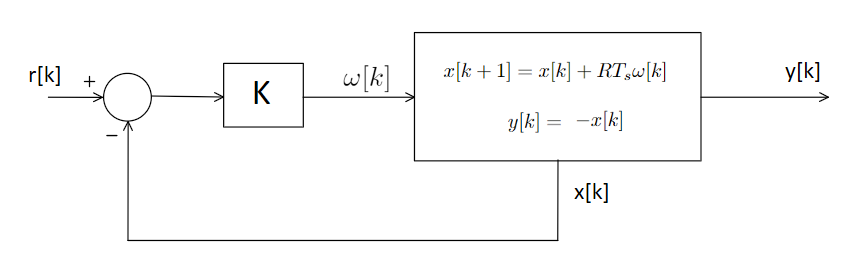
\includegraphics[width=0.7\textwidth]
    {figs/assign3/Q1/vraag3.1.b.png}}
    \caption{Closed-loop system of the state feedback}
    \label{fig:vraag3.1.b feedback}
\end{figure}

\newpar
Applying the stability criterion to the located discrete pole, $|p_d| < 1$, and to the continuous pole, $Re(p_c) < 0$, gives us the boundaries of the stability region of the system. K should satisfy $0<K<\frac{1}{RT_s}$. How the pole moves on a pole-zero map in function of K is illustrated in \autoref{fig:vraag3.1.b_pz}. When increasing K between its allowed boundaries, it moves from the unit circle to the inside on the real axis. In the continuous Laplace-plane, this corresponds to the pole moving from the origin to the left on the negative Real axis. This will make the response of system faster, but also more nervous.  Choosing $K>\frac{1}{RT_s}$ will result in an unstable system. However, there is also a practical limit to K. Increasing K too much will result in saturation of the DC-motors, even before the K hits the stability limit.

\begin{figure}[H]
    \makebox[\textwidth][c]{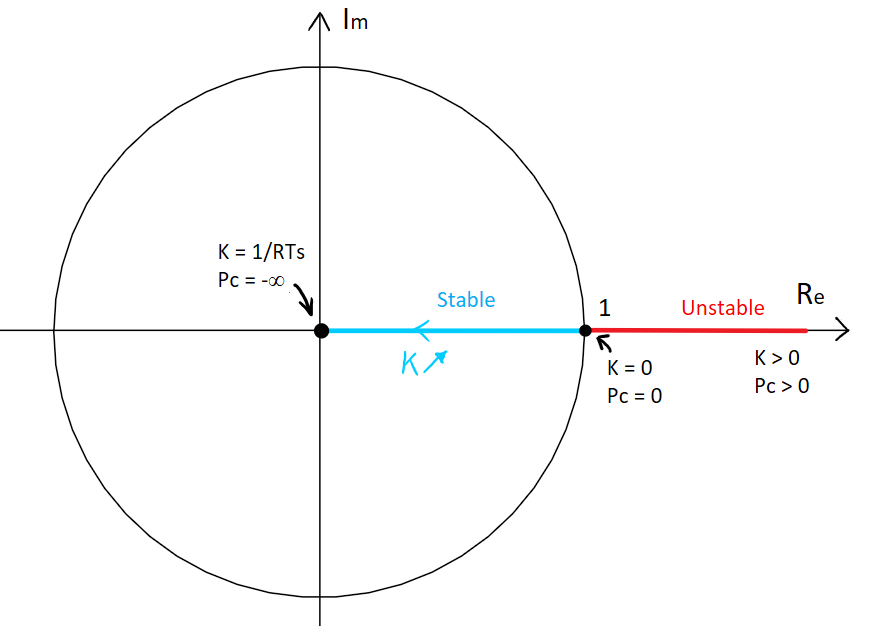
\includegraphics[width=0.7\textwidth]
    {figs/assign3/Q1/vraag3.1.b_pz.png}}
    \caption{PZ-map of the closed-loop system of the state feedback}
    \label{fig:vraag3.1.b_pz}
\end{figure}

\subsection{Validation of Kalman filter principles}
\subsubsection{Measurement equation} 

The discrete measurement equation is shown in \autoref{eq:measurement}

\begin{equation}
    y[k] = Cx[k] + D = -x[k]
    \label{eq:measurement}
\end{equation}

\newpar
So C = -1 and D = 0.

\subsubsection{Expression of \(L_{k+1}\) as function of \(\hat{P}_{k|k}\), Q and R}
\label{section:L_kp1}

Since A, B, C and D are matrices of dimension 1x1, they are considered scalars. Using this results in:

\begin{equation}
    L_{k+1} = \frac{C\hat{P}_{k+1|k}}{S_{k+1}}
\end{equation}

\newpar
Filling in expressions for \(\hat{P}_{k+1|k}\) and \(S_{k+1}\) and using the numerical values of A and C results in:

\begin{equation}
    L_{k+1} = -\frac{\hat{P}_{k|k} + Q_{k}}{\hat{P}_{k|k} + Q_{k} + R_{k+1}}
    \label{eq:2bL}
\end{equation}

\newpar
Letting Q and R consecutively go to \(\infty\) results in the following:

\begin{center}
    \begin{tabular}{p{5cm}p{5cm}}
        \begin{equation}
            \lim_{Q\to\infty} L_{k+1} = -1
            \label{eq:LQinf}
        \end{equation}
        &  
        \begin{equation}
            \lim_{R\to\infty} L_{k+1} = 0
            \label{eq:LRinf}
        \end{equation}
        
    \end{tabular}
\end{center}

\newpar
These results are as expected. If Q becomes large, the trust in the model decreases relative to the trust in the measurement. This leads the estimator to only use measurement data to estimate the position (= state). In other words, the estimation becomes \(x[k+1] = -Ly[k]\).

\newpar
If R becomes large, the trust in the measurement decreases relative to the trust in the model. This leads the estimator to only use the model to estimate the position. In other words, the estimation becomes \(x[k+1] = x[k] + RT_{s}u[k]\).

\subsubsection{Expression of \(\hat{P}_{k+1|k+1}\) as function of \(\hat{P}_{k|k}\), Q and R}

Since A, B, C and D are matrices of dimension 1x1, they are considered scalars. Using this results in:

\begin{equation}
    \hat{P}_{k+1|k+1} = \hat{P}_{k+1|k} + \frac{C^2\hat{P}_{k+1|k}}{S_{k+1}}
\end{equation}

\newpar
Filling in expressions for \(\hat{P}_{k+1|k}\) and \(S_{k+1}\) and using the numerical values of A and C results in:

\begin{equation}
    \hat{P}_{k+1|k+1} = \frac{R_{k+1}\hat{P}_{k|k} + R_{k+1}Q_{k}}{\hat{P}_{k|k} + Q_{k} + R_{k+1}}
    \label{eq:2cP}
\end{equation}

\newpar
Letting Q and R consecutively go to \(\infty\) results in the following:

\begin{center}
    \begin{tabular}{p{6cm}p{6cm}}
        \begin{equation}
            \lim_{Q\to\infty} L_{k+1} = R_{k+1}
            \label{eq:PQinf}
        \end{equation}
        &  
        \begin{equation}
            \lim_{R\to\infty} L_{k+1} = Q_{k} + \hat{P}_{k|k}
            \label{eq:PRinf}
        \end{equation}
        
    \end{tabular}
\end{center}

\newpar
These results are as expected. As said before, when Q becomes large, the estimator only uses measurement data to estimate the position (= state). Therefore the uncertainty of the estimate will equal that of the measurement.

\newpar
Similarly we saw that when R becomes large, the estimator to only uses the model to estimate the position. Therefore the uncertainty of the estimate will equal the model uncertainty.

\subsubsection{Expressions for the steady-state covariance \(\hat{P}_{\infty}\) and related Kalman gain \(L_{\infty}\) as function of Q and R}

If \(k\to\infty\) then \(\hat{P}_{k+1|k+1} = \hat{P}_{k|k} = \hat{P}_{\infty}\). This expression only makes sense if also  \(Q_{k} = Q_{k+1} = Q\) and \(R_{k+1} = R_{k+2} = R\) when \(k\to\infty\) or if Q and R are time independent. Substituting \(\hat{P}_{k+1|k+1}\) and \(\hat{P}_{k|k}\) by \(\hat{P}_{\infty}\) in \autoref{eq:2cP} and rearranging terms results in a second order polynomial:

\begin{equation}
    \hat{P}_{\infty}^2 + Q\hat{P}_{\infty} - QR = 0
\end{equation}

\newpar
This leads to:

\begin{equation}
    \hat{P}_{\infty} = \frac{1}{2} Q \left( \sqrt{1+\frac{4R}{Q}} - 1\right)
    \label{eq:Pinf}
\end{equation}

\newpar
where the negative root was discarded due to the fact that a covariance is always positive.

\newpar
The Kalman gain is found by substituting \(\hat{P}_{k|k} = \hat{P}_{\infty}\) into \autoref{eq:2bL} and then replacing \(\hat{P}_{\infty}\) with \autoref{eq:Pinf}. This results in:

\begin{equation}
    L_{\infty} = -\frac{1+\sqrt{1+\frac{4R}{Q}}}{1+\sqrt{1+\frac{4R}{Q}}+\frac{2R}{Q}}
    \label{eq:Linf}
\end{equation}

\newpar
This steady state Kalman gain should be the same as the fixed LQE gain. The comparison is made in \autoref{tab:LinfLlqe}.

\begin{center}
    \begin{tabular}{ |c|c|c|c|}
    \hline
     Q & R & \(L_{\infty}\) & \(L_{LQE}\) \\
    \hline
    1e-1 & 1e-6 & -1.0000 & -1.0000 \\
    \hline
    1e-6 & 1e-6 & -0.6180 & -0.6180 \\
    \hline
    1e-11 & 1e-6 & -0.0032 & -0.0032 \\
    \hline
    \end{tabular}  
    \captionof{table}{Comparison of the steady-state Kalman gain \(L_{\infty}\) and LQE gain \(L_{LQE}\).}
    \label{tab:LinfLlqe}
\end{center}

\newpar
For each proposed value of Q and R, the estimator gains indeed turn out the same. The behaviour predicted in Section \ref{section:L_kp1} is visible in the table. For relatively larger Q, L becomes -1 and for relative larger R, L becomes small and eventually goes to zero.

\subsubsection{LQE closed loop pole and its behaviour}

The characteristic equation of the LQE is given by:

\begin{equation}
    det\left(s\textbf{I}-\textbf{A}+\textbf{LC}\right) = 0
\end{equation}

\newpar
Because A, L and C are scalar the only eigenvalue is \(s = A-LC\). This is the closed loop pole of the LQE. The estimator is stable if \(A-LC < 0\). Filling in the numerical values for A and C results in:

\begin{equation}
    L < 0
\end{equation}

\newpar
Filling in \autoref{eq:Linf}, which was proven to be an exact representation of the LQE gain, results in:

\begin{equation}
    -\frac{1+\sqrt{1+\frac{4R}{Q}}}{1+\sqrt{1+\frac{4R}{Q}}+\frac{2R}{Q}} < 0
    \label{eq:LQEstab}
\end{equation}

\newpar
Because Q and R are variances, and thus always positive, the condition of \autoref{eq:LQEstab} will always be true. It is thus impossible to make the estimator unstable.

\newpar
The location of the pole in terms of Q and R is:

\begin{equation}
    p_{e} = -\frac{1+\sqrt{1+\frac{4R}{Q}}}{1+\sqrt{1+\frac{4R}{Q}}+\frac{2R}{Q}} = L_{LQE}
    \label{eq:LQEstab}
\end{equation}

\begin{center}
    \begin{tabular}{p{5cm}p{5cm}}
        \begin{equation}
            \lim_{\frac{Q}{R}\to\infty} p_{e} = -1      \label{eq:perhoinf}
        \end{equation}
        &  
        \begin{equation}
            \lim_{\frac{Q}{R}\to0} p_{e} = 0 
            \label{eq:perho0}
        \end{equation}
        
    \end{tabular}
\end{center}

\newpar
For large values of Q/R the pole moves to \( s = -1\). For small values of Q/R the pole moves to \( s = 0\). The estimator thus becomes faster for larger Q/R ratios. This is to be expected since a large Q/R means that the measurement is being trusted more than the model. Therefore the estimated state will react faster on a changing physical state. This effect can clearly be seen in \autoref{fig:varRcteQ} in Section \ref{} 

\subsection{Implementation of state estimator and state feedback controller}
\subsubsection{Choosing values for K and Q}

In order to make a performant estimator and controller, it is important to choose appropriate values for the different design parameters. There are different sources of noise in the system which should be taken into account. $Q$ gives an indication of the process noise, which originates from our our identified model of the cart. This model is accurate (enough), but not perfect. Also the sensor to measure the front distance is not perfect. There will be an error in the measurement with respect to the real distance. The sensor is imperfect, it has a certain resolution and high frequency noise will always be present. This is taken into account by the value $R$. 

\newpar
Choosing an appropriate value of R is relativity straight forward. The sensor is placed at a known distance from a wall, and the sensor output is recorded. Using this data, we can calculate the covariance of the measeruments.

\newpar
To find a good estimation of Q, we have a look at the performance of the state estimator. Plotting the estimated state and the measured distance on the same figure gives us the chance to compare the two. $Q$ should be chosen such that the state is accurate to the measurement, because the sensor is quite trustworthy. However, high frequency noise should be avoided in the estimated state. By lowering $Q$, more trust is given to the model, lowering the influence of the measurements, thus removing noise. When $Q$ is too low, the estimator will lose track of reality, only taking the model into account. It is clear that a balance should be found between these two limit cases.

\newpar
Choosing a value for K again comes down to experimental tuning. When K is too high, overshoot will occur. the cart will pass the reference aimed for, and will have to reverse. Choosing K to low will result in a very slow controller, making the cart approach the reference needlessly slow. It comes down to the designer and the criteria that are subjected on the controller. How much overshoot is allowed? How long do we want the rise time or settling time to be? Again, a balance should be found. More on this in question 3.b. 

\newpar
$P_{0|0}$ tells us the uncertainty of our initial placement of the cart, with respect to the initial estimate. E.g. if we estimate the initial state to be $0.15m$ and we place it down at $0.16m$, the deviation is $0.01m$, making the variance $0.0001m^2$. We estimated our initial placing would be around a cm, so we chose $0.0001m^2$ for $P_{0|0}$.

\newpar
The values we chose for the discussed parameters are shown in \autoref{tab:}


\subsubsection{Influence of feedback constant K on the step response}
In \autoref{fig:vraag3.3.b} the step response of the system is plotted for different values of K. The values of R, Q and $P_{k|k}$ are chosen as listed in \autoref{tab:}. The step input moves the cart from a distance of 15cm to 20 cm. As already mentioned in the previous question, the pole in the feedback system becomes faster when increasing K. This can be recognized in the rise time becoming faster. However, this comes with a pay-off, overshoot is also drastically increased, resulting in a higher settling time. A value of K=55 is chosen to optimize the controller. In our opinion, it provides the smoothest response, minimizing settling time and limiting overshoot.

\begin{figure}[H]
    \makebox[\textwidth][c]{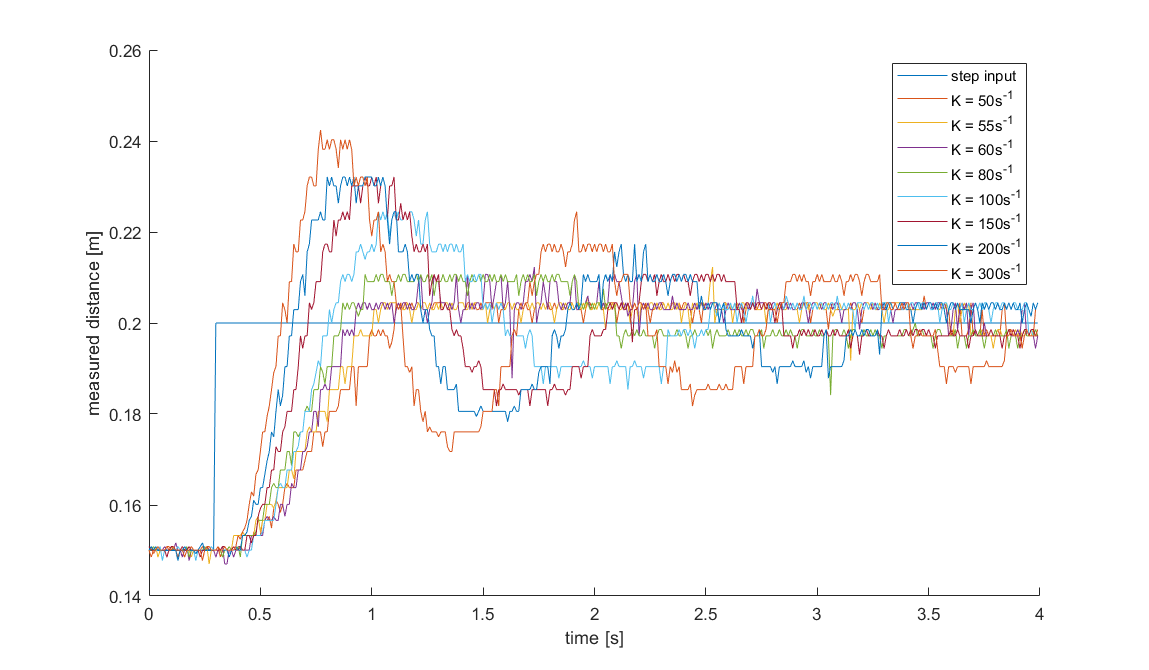
\includegraphics[width=1.15\textwidth]
    {figs/assign3/Q3/vraag3.3.b.png}}
    \caption{Step response of the system with varying feedback constant K}
    \label{fig:vraag3.3.b}
\end{figure}

The control signal of motor A during these experiments are shown in \autoref{fig:vraag3.3.b voltage}. The same remarks made above can be repeated here. Rise time becomes smaller, because the control signal is higher, thus allowing for a faster acceleration of the cart. But again, this comes with a price to pay, overshoot and settling time. It is also important to notice that if K is chosen too high, the motors will be saturated. The control signal will start to exceed the limit of 12 point for a certain K-value. Another limit for K is given by the stability criterion as mentioned in Section \ref{subsec:gain K}

\begin{figure}[H]
    \makebox[\textwidth][c]{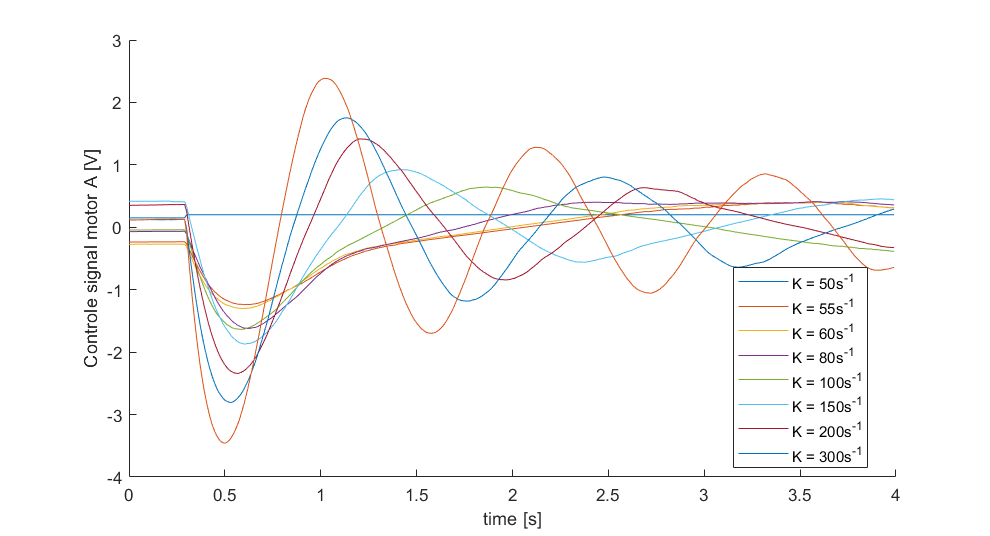
\includegraphics[width=1.15\textwidth]
    {figs/assign3/Q3/vraag3.3.b voltage.png}}
    \caption{Control signal (motor A) of the system during step response with varying feedback constant K}
    \label{fig:vraag3.3.b voltage}
\end{figure}


\subsubsection{Influence of Q and R on the evolution of \(\hat{P}_{k|k}\) and \(L_{k}\)}
To analyse the influence of Q and R on \(\hat{P}_{k|k}\) and \(L_{k}\), the cart is positioned at a distance of 30cm. When the controller and estimator are enabled, the reference distance is set to 15 cm. Two sets of measurements were made. The first one keeps R at a constant value of \(R=9.5199m^2\), varying Q between 1e-1 and 1e-11\(m^2\). The results are visualised in the upper half of \autoref{fig:vraag3.3.c_PL}. The second set shows data for Q constant and equal to 1e-8\(m^2\), with R varying from 1 to 1e-6\(m^2\) . Results are plotted in the lower half of \autoref{fig:vraag3.3.c_PL}.

\begin{figure}[H]
\begin{adjustwidth}{-3cm}{-3cm}
\centering
\begin{tabular}{cc}
  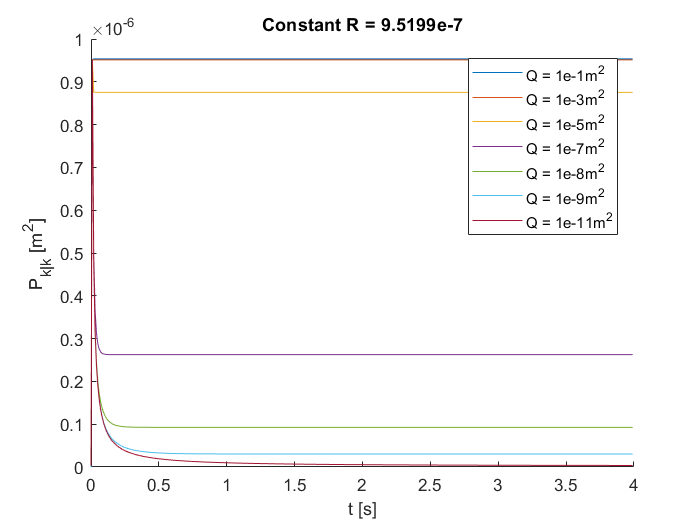
\includegraphics[width=80mm]{figs/assign3/Q3/vraag3.3.c_RP.png} &   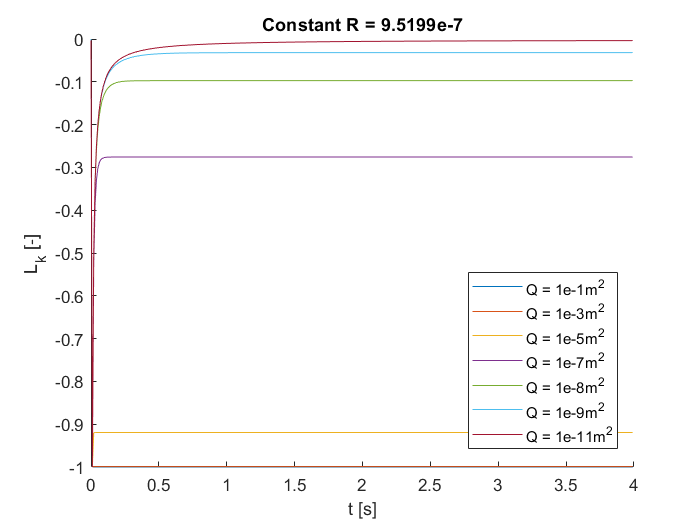
\includegraphics[width=80mm]{figs/assign3/Q3/vraag3.3.c_RL.png} \\
  
  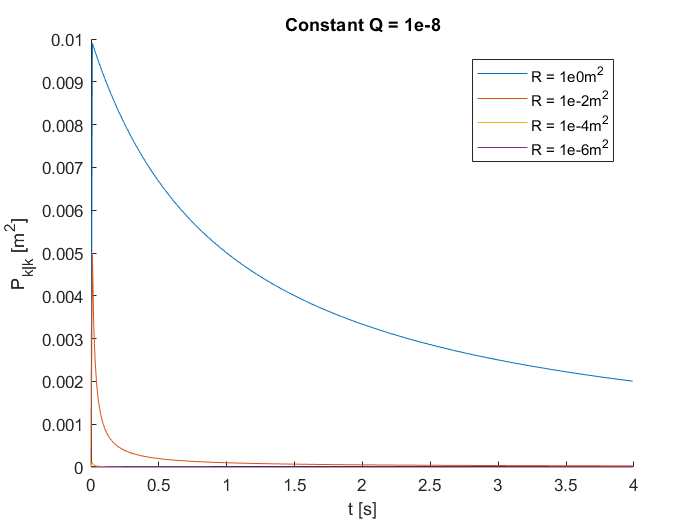
\includegraphics[width=80mm]{figs/assign3/Q3/vraag3.3.c_QP.png} & 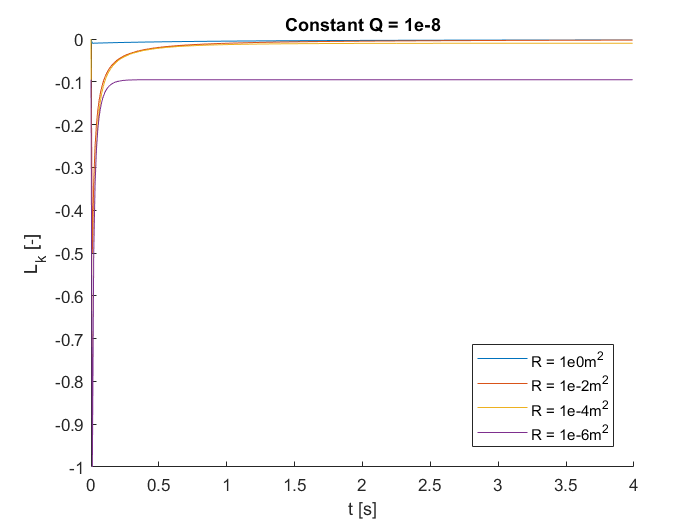
\includegraphics[width=80mm]{figs/assign3/Q3/vraag3.3.c_QL.png} \\
\end{tabular}
\end{adjustwidth}
\captionof{figure}{The evolution of \(\hat{P}_{k|k}\) and \(L_{k}\) for different values of Q and R}
\label{fig:vraag3.3.c_PL}
\end{figure}

\newpar
These results are in line with the answers given in question 2(e) and 2(d). In 2(e) the remark was made that an estimator with a large Q/R ratio is faster than one with a low Q/R ratio. The same can be noticed in \autoref{fig:vraag3.3.c_PL}. Both \(\hat{P}_{k|k}\) and \(L_{k}\) reach their constant value sooner when Q/R is large. 

\newpar
The results are also consistent with the answers given in 2(d).
In \autoref{} a few values of \(L_\infty\) are listed for some of the Q and R values used in the experiments. The third column shows the value when calculated with the expression obtained in 2(d). The fourth column lists the values of L after it has stabilised in the experiments. It is clear these correspond to each other as they are almost always exactly the same.

\begin{center}
    \begin{tabular}{ |c|c|c|c|}
    \hline
    R [\(m^2\)] & Q [\(m^2\)] & \(L_\infty\) calculated [-] & \(L_\infty\) measured [-]  \\
    \hline
    9.5199e-7        & 1e-1     & -0.99999      &   -0.99999           \\
    \hline
    9.5199e-7        & 1e-3     & -0.99904      &  -0.99905                 \\
    \hline
    9.5199e-7        & 1e-5     & -0.91950      &  -0.91950            \\
    \hline
    9.5199e-7        & 1e-7     & -0.27581      & -0.27581           \\ 
    \hline
    9.5199e-7        & 1e-8     & -0.09737      & -0.09737           \\ 
    \hline
    9.5199e-7        & 1e-9     & -0.03188      & -0.03188           \\ 
    \hline
    9.5199e-7        & 1e-11    & -0.00323      & -0.00376           \\ 
    \hline
    \end{tabular}  
    \captionof{table}{location and frequency of poles and zeros in the fitted system}
    \label{tab:location_Sys_31z_f}
\end{center}


\subsubsection{Kalman filter consistency: NIS and SNIS}

The NIS and SNIS are calculated as follows (values of A, B and C filled in):

\begin{equation}
    NIS_{k}=\nu_{k} S_{k}^{-1} \nu_{k} = \frac{\left[y_{k}+\left( \hat{x}_{k-1|k-1}+R T_{s} u_{k-1}\right)\right]^{2}}{\left( \hat{P}_{k-1|k-1}+Q_{k-1}\right)+R_{k}}
    \label{eq:nis}
\end{equation}

\newpar
with \(y\) the measured distance and \(u\) the desired velocity. The state estimate covariance $\hat{P}$, state estimate $\hat{x}$ and $u$ are essential ti the functioning of the controller and are calculated ever time step. They can always be recorded in an experiment. The same is true for the measurement $y$. The controller also calculates $\nu$ and $S$ as intermediate steps for the calculations. They can also be recorded. Both formulations of the NIS can thus be used starting from the recorded measurement data.

\begin{equation}
    SNIS_{k}=\sum_{j=k-M+1}^{k} NIS_{j}
    \label{eq:snis}
\end{equation}

\newpar
The SNIS can be calculated out of the calculated NIS values as illustrated in \autoref{eq:snis}. In this section M is chosen to be 5.

\newpar
The expected probability density of the NIS is $\chi^2$. In the numerator of equation \autoref{eq:nis} three gaussian random variables, namely $y$, $\hat{x}$ and $u=f(\hat{x})$ (due to feedback). The sum of these random variables, which is also a gaussian distribution, is then squared, resulting in a $\chi^2$ distribution.

\newpar
The SNIS is a $\chi^2$ distribution of degree M (degree 5 in this section). This is the result of the summation of M $\chi^2$ distributed NIS values to obtain the SNIS.

\newpar
The consistency is checked using confidence intervals. The confidence bounds $\alpha_{1}$ and $\alpha_{2}$ for e.g. an $95\%$ confidence interval are determined as:

\begin{center}
    \begin{tabular}{ccc}
        \(0.025 = F_{\chi^2_{M}}(\alpha_{1})\) &   and    & \(0.975 = F_{\chi^2_{M}}(\alpha_{2})\)
    \end{tabular}
\end{center}

\newpar
With \(F_{\chi^2_{M}}(\alpha)\) the cumulative distribution corresponding to the $\chi^2$ distribution of degree M. 
If R is measured and Q chosen correctly and the assumption of gaussian measurement noise and process noise hold, the innovation should be gaussian distributed to. In that case the percentage of NIS or SNIS points between the confidence bounds should exactly match the value for which the bounds are calculated, here $95\%$. If the statistical model does not match with reality, less (S)NIS point will lie in the interval. A greater discrepancy in the percentage results in lower confidence in the statistical model and thus in a lower consistency between the model and the real world.
    

\newpar
!!!!!!!!!!!!!!! UNITS R AND Q !!!!!!!!!!!!!!!

\begin{figure}[H]
\begin{adjustwidth}{-3cm}{-3cm}
\centering
\begin{tabular}{cc}
  \includegraphics[width=80mm]{figs/assign3/Q3/Qe_1.png} &   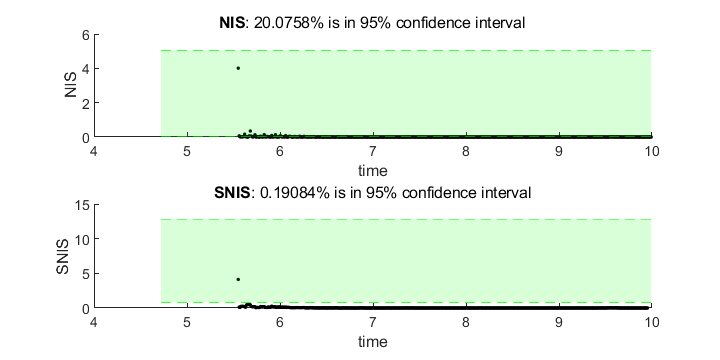
\includegraphics[width=80mm]{figs/assign3/Q3/Qe_3.png} \\
  Q = 1e-1, R = 9.52e-7 & Q = 1e-3, R = 9.52e-7 \\[8pt]
  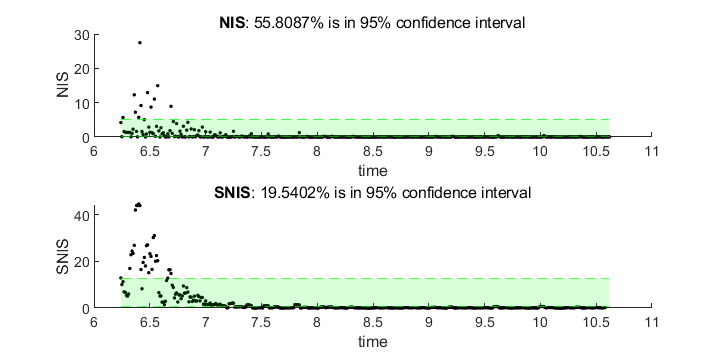
\includegraphics[width=80mm]{figs/assign3/Q3/Qe_5.png} & \includegraphics[width=80mm]{figs/assign3/Q3/Q95199e_11.png} \\
  Q = 1e-5, R = 9.52e-7 & Q = 1e-6, R = 9.52e-7 \\[8pt]
  \includegraphics[width=80mm]{figs/assign3/Q3/Qe_7.png} & 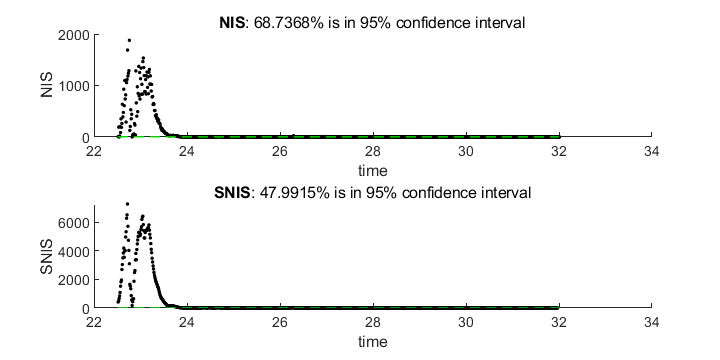
\includegraphics[width=80mm]{figs/assign3/Q3/Qe_8.png} \\
  Q = 1e-7, R = 9.52e-7 & Q = 1e-8, R = 9.52e-7 \\[8pt]
  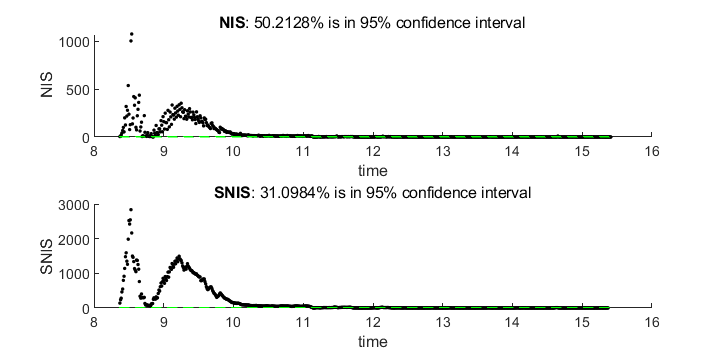
\includegraphics[width=80mm]{figs/assign3/Q3/Qe_9.png} & \includegraphics[width=80mm]{figs/assign3/Q3/Qe_11.png}\\
  Q = 1e-9, R = 9.52e-7 & Q = 1e-11, R = 9.52e-7
\end{tabular}
\end{adjustwidth}
\captionof{figure}{NIS and SNIS for varying values of Q and constant value of R = 9.52e-7.}
\label{fig:QcteR}
\end{figure}


\begin{figure}[H]
\begin{adjustwidth}{-3cm}{-3cm}
\centering
\begin{tabular}{cc}
  \includegraphics[width=80mm]{figs/assign3/Q3/Re_0.png} &   \includegraphics[width=80mm]{figs/assign3/Q3/Re_2.png} \\
  Q = 1e-8, R = 1e-0 & Q = 1e-8, R = 1e-2 \\[8pt]
 \includegraphics[width=80mm]{figs/assign3/Q3/Re_4.png} &   \includegraphics[width=80mm]{figs/assign3/Q3/Re_6.png} \\
 Q = 1e-8, R = 1e-4 & Q = 1e-8, R = 1e-6 \\[8pt]
\end{tabular}
\end{adjustwidth}
\captionof{figure}{NIS and SNIS for varying values of R and constant value of Q = 1e-8.}
\label{fig:cteQR}
\end{figure}

\begin{figure}[H]
    \centering
    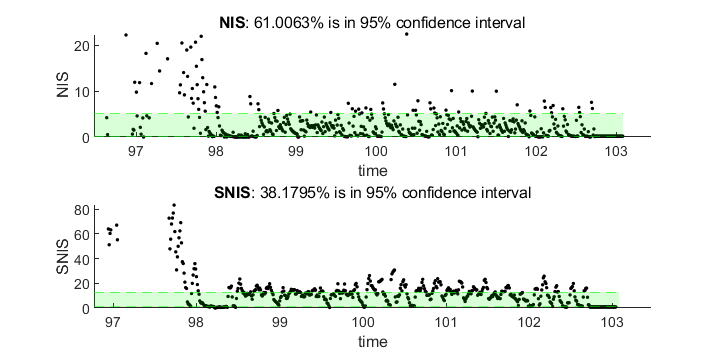
\includegraphics[width=100mm]{figs/assign3/Q3/Re_6_zoom.png}
    \captionof{figure}{\centering Enlarged view of the Q and R setting which comes closest to consistency: Q=1e-8, R=1e-6}
    \label{fig:zoomconsistent}
\end{figure}

\newpar
The resulting NIS and SNIS are plotted above in \autoref{fig:QcteR} and \autoref{fig:cteQR}. \autoref{fig:QcteR} shows the results for a constant R of $9.52e-7$ and different values of Q, going from a to large Q to a to small Q. The overall best result is there found for Q = 1e-8, but in none of the cases the Kalman filter is consistent. \autoref{fig:cteQR} shows the results for a constant Q of 1e-8 and different values of R. Here too the overall best result is found for $R = 1e-6 \approx 9.52e-7$. 

\newpar
\autoref{fig:zoomconsistent} shows an enlarged view of the NIS and SNIS for Q=1e-8 and R=1e-6, cutting away the transient and focusing in the steady state results. Of all the experiments, this one comes closest to consistency. Especially the NIS points are quite good located within the confidence bounds. Their distribution also starts to become random, as would be expected from a consistent filter.

\newpar
The inconsistency of the filter is generally due to deviations on the assumed statistical behaviour, like correlated noise sources or deterministic modeling errors. For example non linear system behaviour in the transient will cause a deterministic error between the model and the real world, causing the NIS and SNIS to be highly deterministic and also show a transient. This effect is visible in the plots made above. Related to this, it is virtually impossible to make a good estimate for Q, since it is an artificial quantity to fix random deviations of the system compared to the model. Q can be tuned to let the filter come close to consistency, but it will never be consistent if the modeled statistics do not correspond to the real world. 


\subsubsection{Influence or Q/R ration on the position estimate}
The results of the demanded experiments are visualised in \autoref{fig:QcteR_state_respons} and \autoref{fig:cteQR_state_respons}. The plots in the figures are arranged from large to small $\rho$ = Q/R ratio. It is clear that the estimator converges faster to the measurements for larger Q/R ratios. R is a measure for the uncertainty of the measured state. Thus if R is small, the measurements are trusted a lot. Q is a measure for the uncertainty of the calculated state based on the model. When this uncertainty is large, the correctness of the model is doubted. 

\newpar
Combining these interpretations explains the results. A large Q/R ratio means little trust is given to the model, and a lot of trust is given to the measurements, thus converging to the measurements faster. 

\begin{figure}[H]
\begin{adjustwidth}{-3cm}{-3cm}
\centering
\begin{tabular}{cc}
  \includegraphics[width=80mm]{figs/assign3/Q3/33e/Qe_1.png} & \includegraphics[width=80mm]{figs/assign3/Q3/33e/Q95199e_11.png} \\
  Q = 1e-1, R = 9.52e-7 $\implies \rho$ = 1.1e5 & Q = 1e-6, R = 9.52e-7 $\implies \rho$ = 1.1e-0\\[8pt]
  \includegraphics[width=80mm]{figs/assign3/Q3/33e/Qe_7.png} & \includegraphics[width=80mm]{figs/assign3/Q3/33e/Qe_11.png} \\
  Q = 1e-7, R = 9.52e-7 $\implies \rho$ = 1.1e-1 & Q = 1e-11, R = 9.52e-7 $\implies \rho$ = 1.1e-5
\end{tabular}
\end{adjustwidth}
\captionof{figure}{Estimated state evolution and actual measurement for wrong initial position estimate. Effect of varying Q (with constant value of R = 9.52e-7).}
\label{fig:QcteR_state_respons}
\end{figure}


\begin{figure}[H]
\begin{adjustwidth}{-3cm}{-3cm}
\centering
\begin{tabular}{cc}
  \includegraphics[width=80mm]{figs/assign3/Q3/33e/Re_6.png} & \includegraphics[width=80mm]{figs/assign3/Q3/33e/Re_4.png}\\
  Q = 1e-8, R = 1e-6 $\implies \rho$ = 1e-2 & Q = 1e-8, R = 1e-4 $\implies \rho$ = 1e-4\\[8pt]
  \includegraphics[width=80mm]{figs/assign3/Q3/33e/Re_2.png} & \includegraphics[width=80mm]{figs/assign3/Q3/33e/Re_0.png}\\
  Q = 1e-8, R = 1e-2 $\implies \rho$ = 1e-6 & Q = 1e-8, R = 1e-0 $\implies \rho$ = 1e-8\\[8pt]
\end{tabular}
\end{adjustwidth}
\captionof{figure}{Estimated state evolution and actual measurement for wrong initial position estimate. Effect of varying R (with constant value of Q=1e-8).}
\label{fig:cteQR_state_respons}
\end{figure}

\subsubsection{System behaviour using slow pole placement estimator}

The closed loop continuous time pole of the state feedback controller is $P_{c,c} = -(BK-A)$. The discrete pole of the estimator that is ten times slower then the controller is thus:

\begin{equation}
    P_{e,d} = e^{-T_{s}\frac{\left(BK-A\right)}{10}}
\end{equation}

\newpar
Using the continuous time A = 0, B = 1 and the above used value for the feedback K = 55, $P_{e,d}$ calculated and L is calculated using acker in matlab:

\begin{equation}
    L = acker(A,AC,P_{e,d})
\end{equation}

\nawpar
using the discrete time A = 1 and C = -1. The numerical results are:

\begin{center}
    \begin{tabular}{|c|c|}
        \hline
        $P_{e,d}$ & 0.9982 \\
        \hline
        L & -0.0018 \\
        \hline
    \end{tabular}
\end{center}

\newpar
Implementing this estimator and giving it a wrong initial estimate results in the following dynamic behaviour:

\begin{figure}[H]
    \centering
    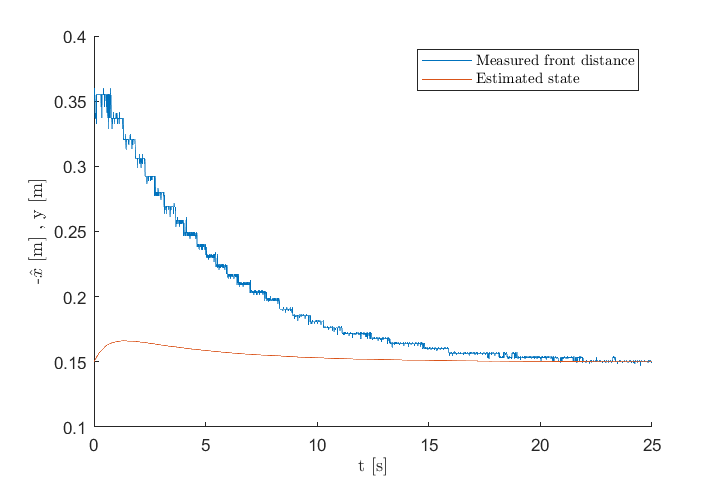
\includegraphics[width=120mm]{figs/assign3/Q3/vraag3f.png}
    \captionof{figure}{\centering State evolution using pole placement estimator with L=-0.0018. The estimator is ten times slower than the feedback controller.}
    \label{fig:poleplacementcontrollerstate}
\end{figure}




\end{document}
